\sectionframe{Label Distribution Smoothing (LDS)}
\begin{frame}{Imbalanced Categorical vs. Continuous Label Space (1/3)}
	\begin{tikzpicture}[remember picture, overlay]
		\node[right=0.28\textwidth,below=2em] at (current page.north west) 
		{
			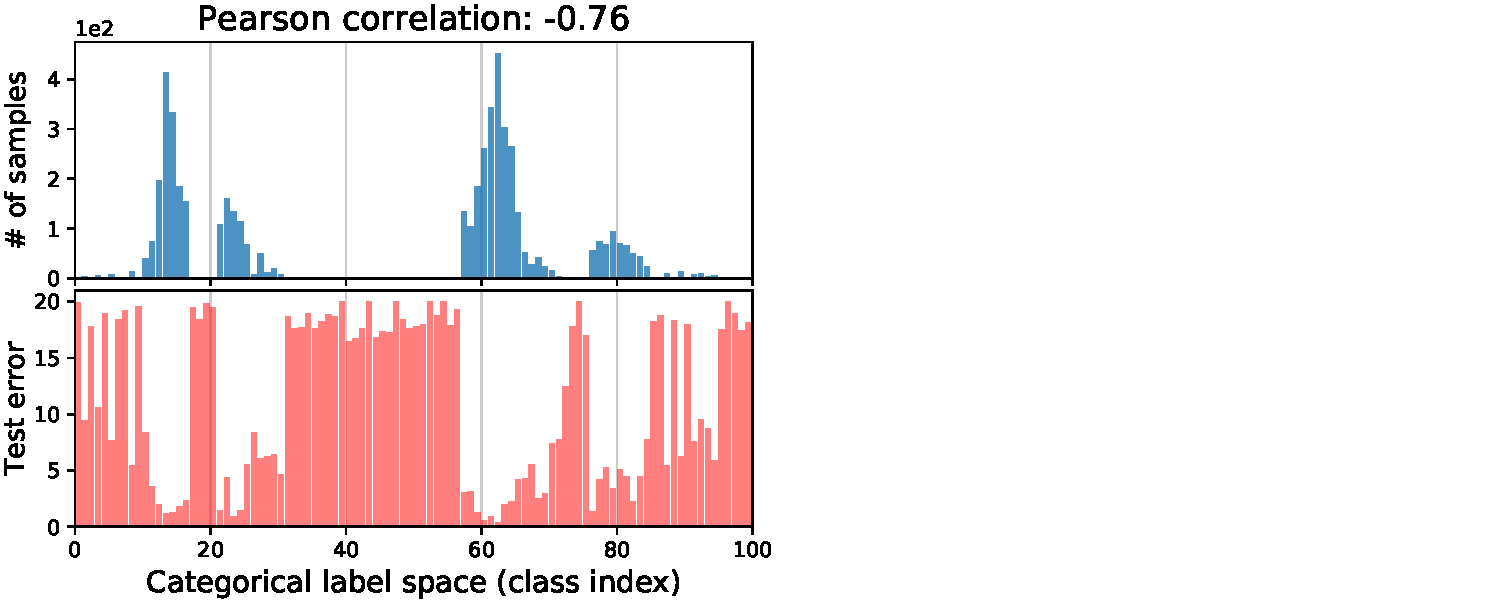
\includegraphics[width=0.5\textwidth]{images/err_motivate_1_left.pdf}
		};
		\node[left=0.25\textwidth,below=2em] at (current page.north east) 
		{
			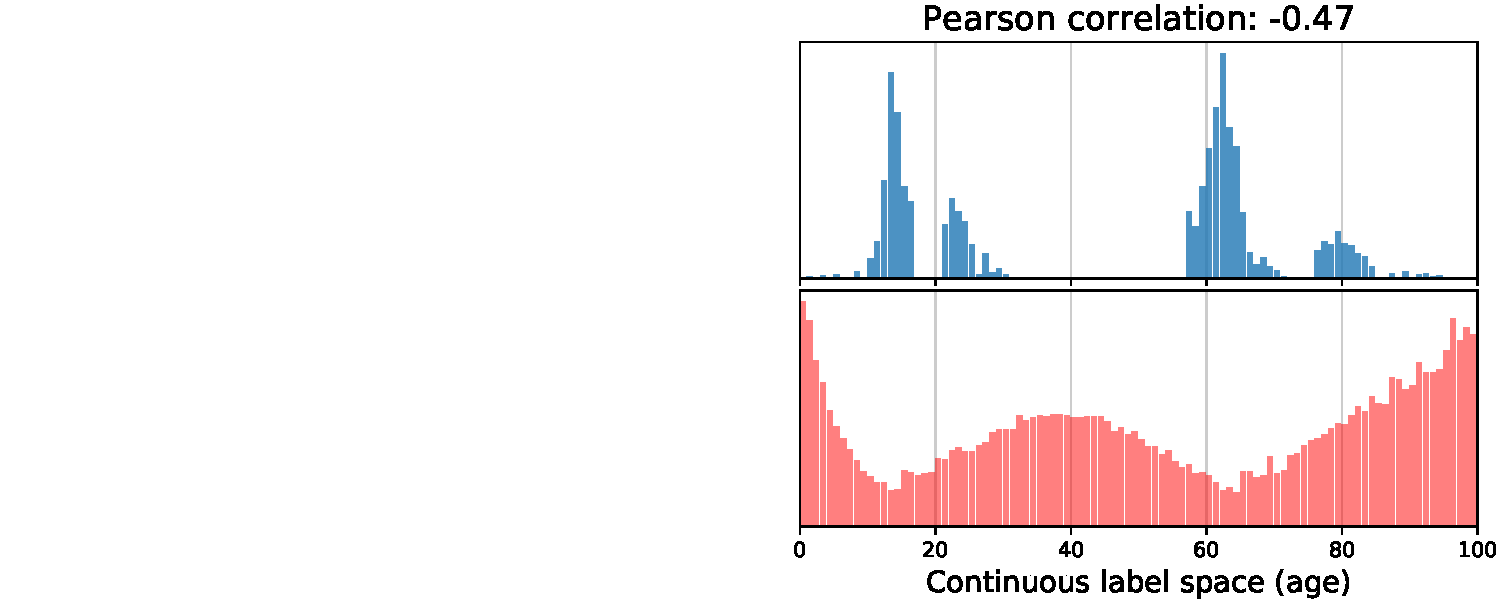
\includegraphics[width=0.46\textwidth]{images/err_motivate_1_right.pdf}
		};
	\end{tikzpicture}
	\vspace{0.45\textheight}
	\begin{columns}[T]\footnotesize
		\begin{column}{0.5\textwidth}
			\begin{itemize}
				\item task: picture $\longrightarrow$ class
				\item data souce: CIFAR-100
			\end{itemize}
		\end{column}
		\begin{column}{0.5\textwidth}
			\begin{itemize}
				\item task: \\person's picture $\longrightarrow$ person's age
				\item age subrange: 0-99
				\item data souce: IMDB-WIKI
			\end{itemize}
		\end{column}
	\end{columns}
	\vspace{1em}
	\begin{itemize}\footnotesize
		\centering\item Simulated label imbalance
		\centering\item Label density distributions forced to be equal
		\centering\item Balanced test sets
	\end{itemize}
	\credit{Image}{yang2021delving}
\end{frame}

\begin{frame}{Imbalanced Categorical vs. Continuous Label Space (2/3)}
	\begin{tikzpicture}[remember picture, overlay]
		\node[right=0.28\textwidth,below=2em] at (current page.north west) 
		{
			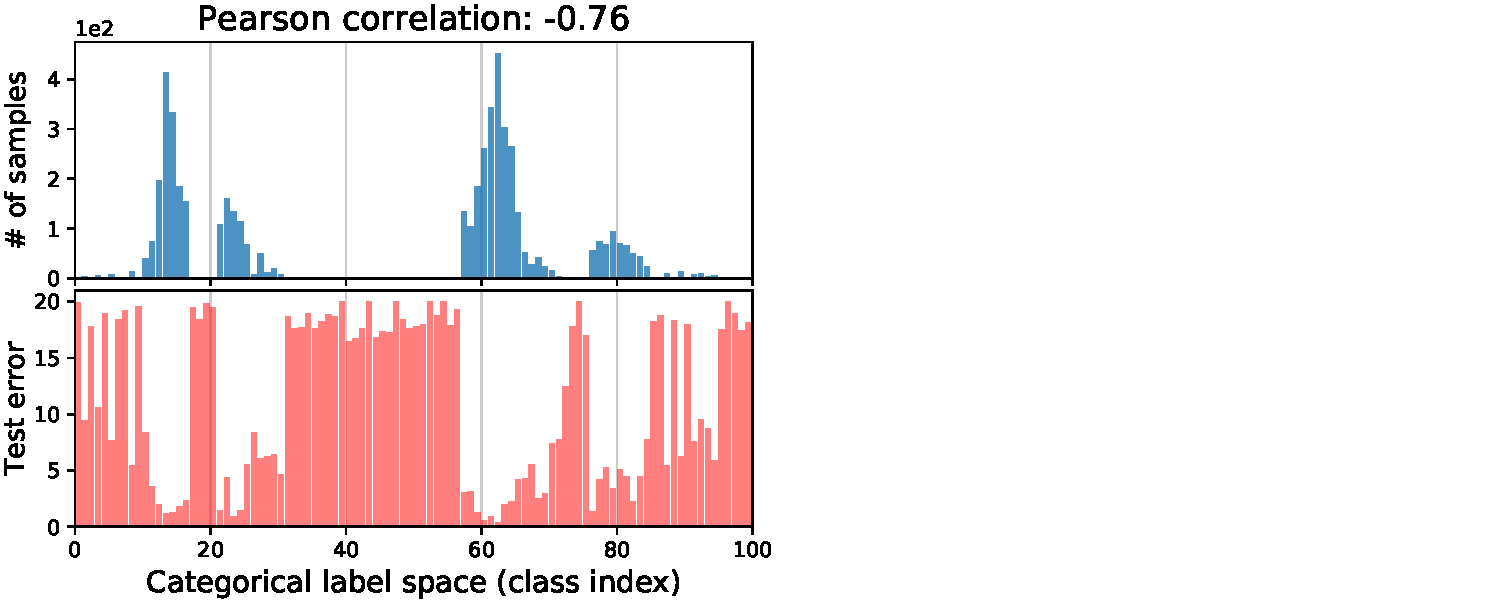
\includegraphics[width=0.5\textwidth]{images/err_motivate_1_left.pdf}
		};
		\node[left=0.25\textwidth,below=2em] at (current page.north east) 
		{
			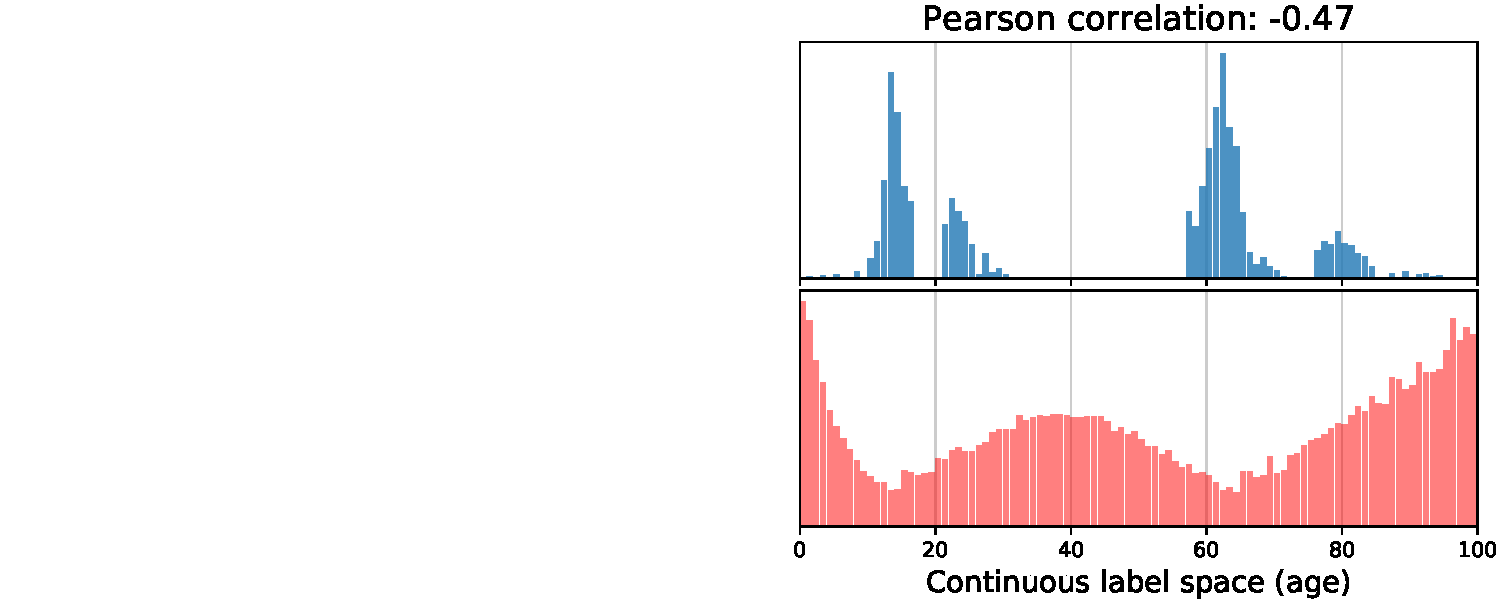
\includegraphics[width=0.46\textwidth]{images/err_motivate_1_right.pdf}
		};
	\end{tikzpicture}
	\vspace{0.45\textheight}
	\begin{columns}[T]\footnotesize
		\begin{column}{0.5\textwidth}
			\begin{itemize}
				\item error distribution \emph{correlates} with label density distribution
				\item<2-> majority classes with more examples are better learned than minority classes
			\end{itemize}
		\end{column}
		\begin{column}{0.5\textwidth}
			\begin{itemize}
				\item error distribution DOES NOT \emph{correlate} well with label density distribution
				\item<2-> smoother error distribution
			\end{itemize}
		\end{column}
	\end{columns}
	\credit{Image}{yang2021delving}
\end{frame}

\begin{frame}{Imbalanced Categorical vs. Continuous Label Space (3/3)}
	\begin{tikzpicture}[remember picture, overlay]
		\node[right=0.28\textwidth,below=2em] at (current page.north west) 
		{
			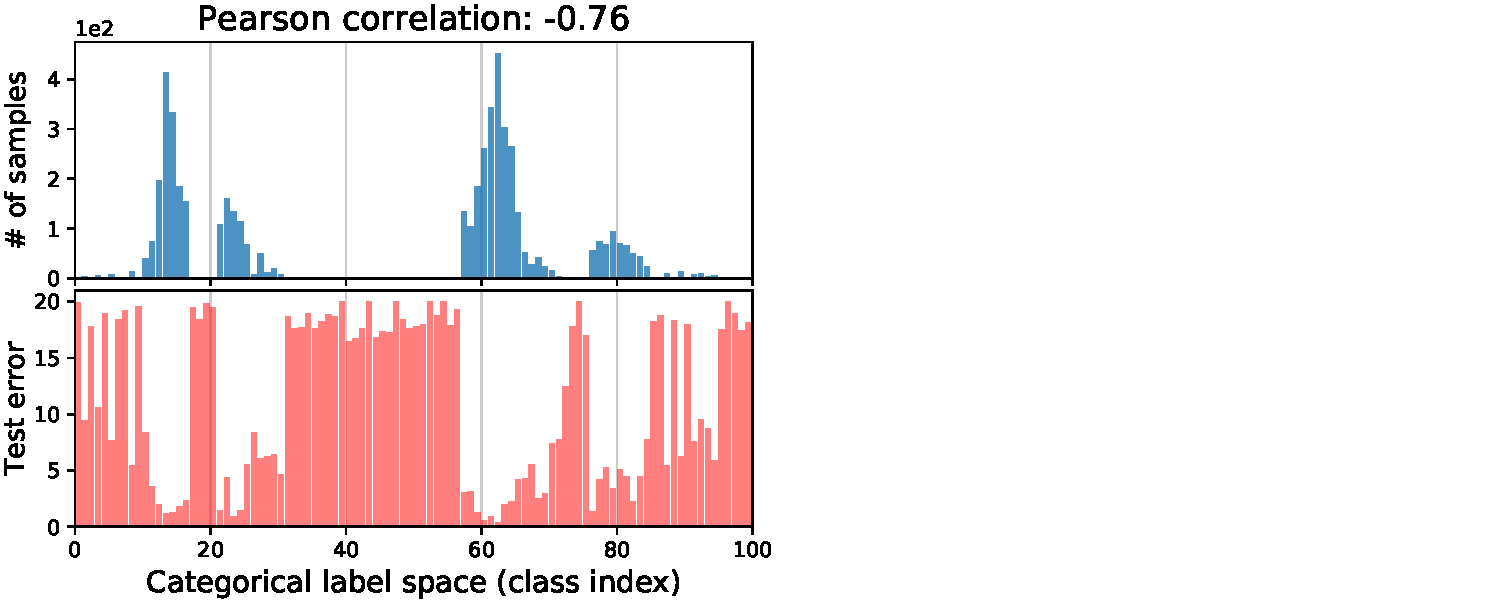
\includegraphics[width=0.5\textwidth]{images/err_motivate_1_left.pdf}
		};
		\node[left=0.25\textwidth,below=2em] at (current page.north east) 
		{
			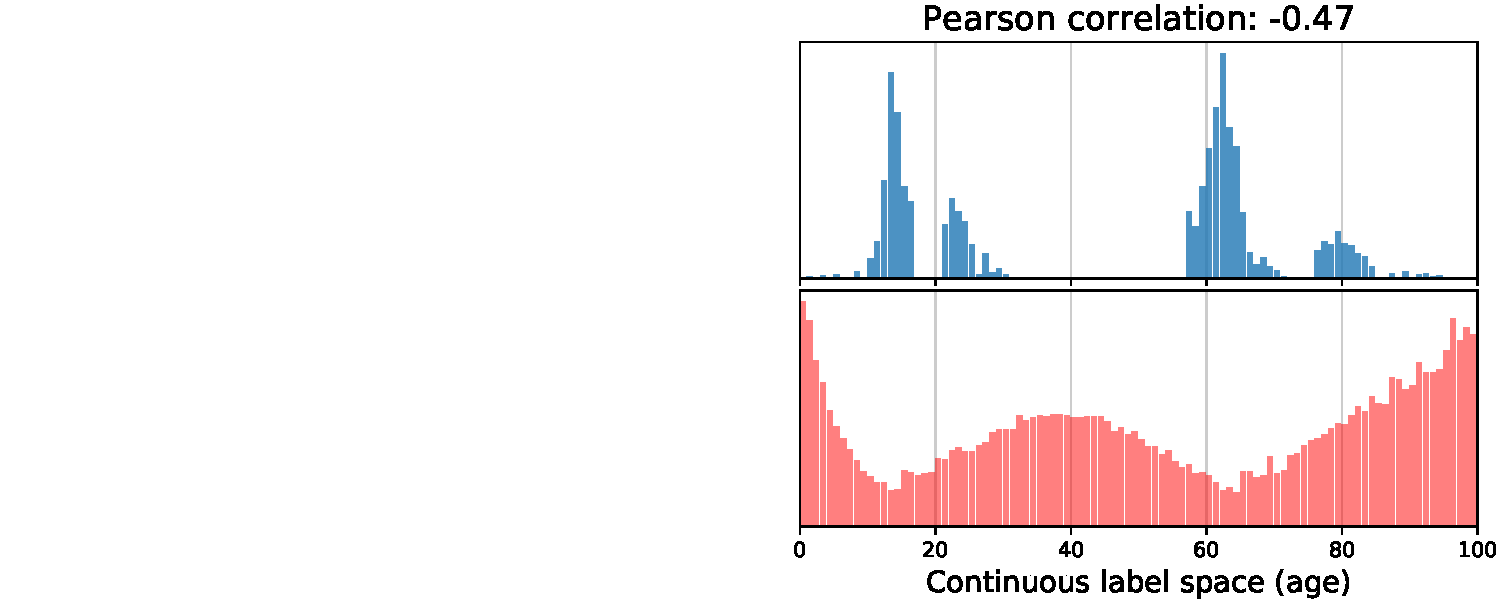
\includegraphics[width=0.46\textwidth]{images/err_motivate_1_right.pdf}
		};
	\end{tikzpicture}
	\vspace{0.45\textheight}
	\begin{columns}[T]\footnotesize
		\fontsize{7pt}{7.2}\selectfont
		\begin{column}{0.5\textwidth}
			\begin{itemize}
				\item Compensating for imbalance in empirical label
				density distribution WORKS WELL.
			\end{itemize}
		\end{column}
		\begin{column}{0.5\textwidth}
			\begin{itemize}\setlength\itemsep{.5em}
				\item Compensating for imbalance in empirical label
				density distribution is INACCURATE.
				\item Empirical density does not accurately reflect imbalance as seen by model.
				\item<2-> Intuition: dependence between features at nearby labels.
				\item<2-> Proposed solution: \\\textbf{Label Distribution Smoothing (LDS)}
			\end{itemize}
		\end{column}
	\end{columns}
	\credit{Image}{yang2021delving}
\end{frame}

\begin{frame}{Label Distribution Smoothing (LDS) - Overview}
	\begin{figure}[h]
		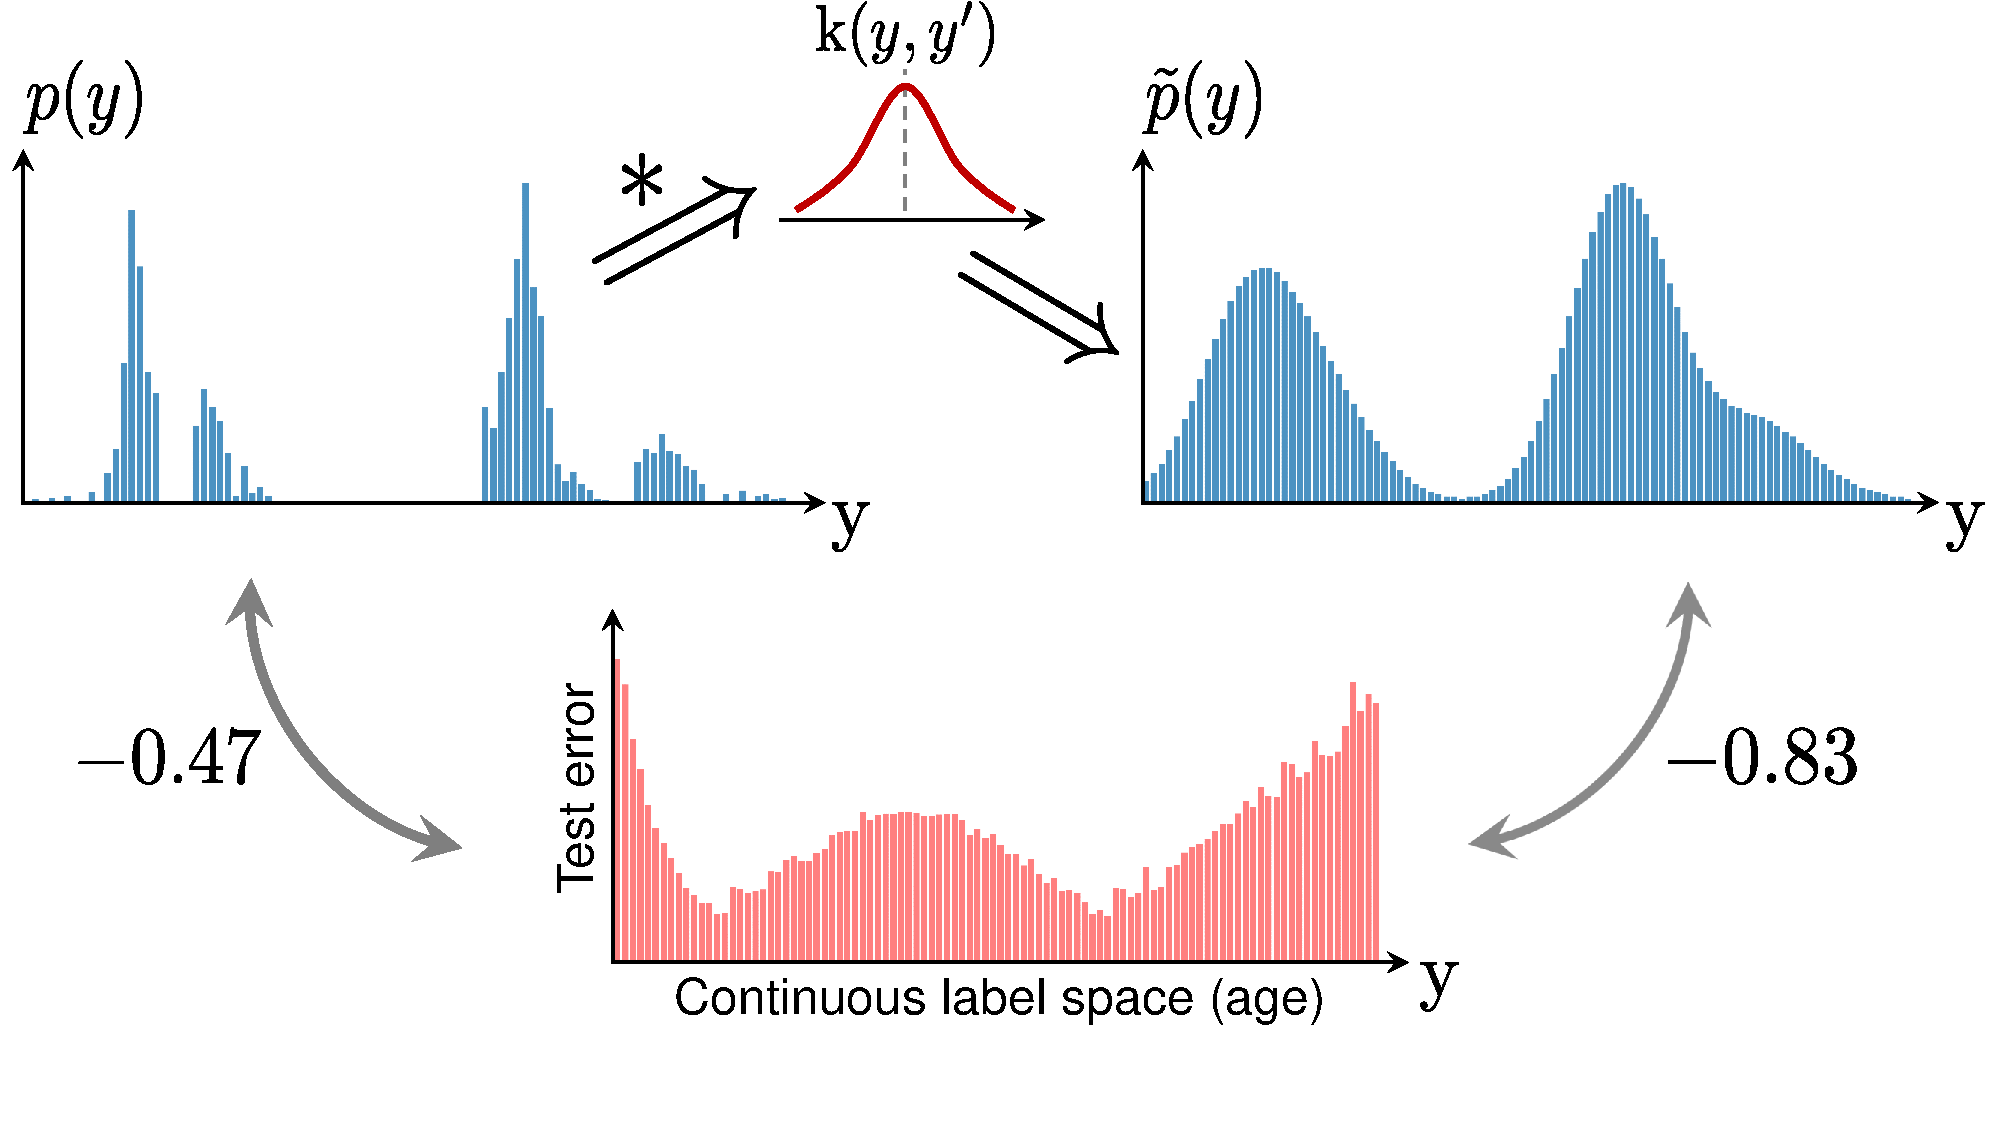
\includegraphics[width=\linewidth]{images/err_motivate_sep.pdf}
		%\caption{}
	\end{figure}
	\credit{Image}{yang2021delving}
\end{frame}

\begin{frame}[shrink=3]{Label Distribution Smoothing (LDS)}
	\begin{itemize}\setlength\itemsep{.5em}
		\item<1-> Starting points
		\begin{itemize}
			\item Dependence between features at nearby continuous labels.
			\item Expected density estimation
			\begin{itemize}
				\item Significant literature in statistics~(\cite{parzen1962estimation})
				\item Kernel density estimation
			\end{itemize}
		\end{itemize}
		\item<2-> Functioning
		\begin{itemize}
			\item Convolves symmetric kernel with empirical label density distribution.
			\item Extracts kernel-smoothed label density accounting for feature overlap of neighbouring labels.
		\end{itemize}
		\item<3-> Symmetric kernel
		\begin{itemize}
			\item E.g., Gaussian, Laplacian, triangular kernel.
			\item Similarity between target values w.r.t. their distance in target space.
		\end{itemize}
		\item<4-> \emph{Effective label density distribution}
		\begin{equation*}
			\tilde{p}(y') \triangleq \int_\mathcal{Y} k(y,y')p(y)dy
		\end{equation*}
		where 
		\begin{itemize}
			\item $p(y)$: nr. occurrences of label $y$ in training data.
		\end{itemize}
		\item<5-> Usage
		\begin{itemize}
			\item Possible direct adaptation of class imbalance techniques.
			\item E.g., loss weighted by inverse effective label density.
		\end{itemize}
	\end{itemize}
\end{frame}